% !TEX TS-program = pdflatexmk-c
\documentclass[11pt, letterpaper]{article}

\usepackage[brazilian, english]{babel}
\usepackage[utf8]{inputenc}
\usepackage[T1]{fontenc}
\usepackage[draft]{todonotes}   % notes showed
\usepackage{geometry}
\usepackage{lipsum}
\usepackage{enumitem}
\usepackage{float}
\usepackage{forest}

\usepackage{csvsimple}
\usepackage{array}

\usepackage{multicol}

% set custom date and format
\usepackage[nodayofweek,level]{datetime}
\newcommand{\mydate}{\formatdate{17}{3}{2016}}
\newdateformat{mydateformat}{ \THEMONTH \dateseparator \THEDAY \dateseparator \THEYEAR}

%bibliography
\usepackage[backend=biber, bibencoding=utf8,style=numeric]{biblatex}
\addbibresource{bibfile.bib}
\appto{\bibfont}{\scriptsize} % \footnotesize

\title{\vspace{-2cm} 19702 \\ Project 1}
\author{Francisco Fonseca \and Octavio Mesner}
\date{\mydate}

\date{\mydateformat\normalsize\mydate} % Today's date or a custom date

\begin{document}

% \maketitle % Print the title

\section*{Executive Summary} \label{execsum}

\pagebreak
\section{Introduction} \label{intro}

New York City (NYC) would like to implement a fleet of autonomous
vehicles (AV) by 2020 as part of a larger initiative of establishing
itself as a world leader in smart city infrastructure. AV is a fledgling technology
that has seen tremendous advances in recent years involving
big technology players such as Google and Uber. An AV vehicle is equiped with
GPS, radar sensors and computer processors which enable it to drive itself without the
need of human interaction. Because of the
novel nature of AV technology, there is a considerable amount of
uncertainty regarding the impact of its implementation on traffic
issues including safety, congestion, energy consumption and environmental impacts.
NYC officials wish to study potential alternatives and determine their effect, while
considering uncertainty, on these outcome
and optimal strategies moving forward with AV
technology within the NYC fleet of vehicles. This study will focus on
the alternatives available to implement  this technology
from AutoMerge, Inc. (AM) specifically in NYC's 40-passenger transit
buses. It will compare different alternative strategies by performing
a Benefit Cost Analysis (BCA) to assess how these different options
impact the general population of NYC, which are the main stakeholders
in this issue. Among the factors to be included in the analysis are:
safety, energy consumption, air pollution, GHG emissions, weather
conditions and time savings due to improvement in traffic flow. Section \ref{problem}
presents a detailed description of the problem and the alternatives analyzed. Section
\ref{results} presents the analysis of each alternative and the
results found. In section \ref{sensitivity} a sensitivity analysis is
performed for some inputs. Section \ref{discussion} discusses the
results of the analyses and section \ref{conclusion} presents the
conclusion and recommendations of this study.

\section{Problem Description} \label{problem}
\subsection{Alternatives}

Broadly, NYC must consider the following three alternatives.

\begin{description}[leftmargin=0pt]
\item[Alternative 1:] Do not implement AV.

This is the reference alternative. AV is not implemented and the
benefits and costs are the ones already incurred to the population.
There is relatively little uncertanty associated with this outcome
because there is historical data to project the effect of this
alternative on outcomes.

\item[Alternative 2:] Implement AV in the NYC bus fleet.

In this alternative, the city implements the AV technology in the bus
fleet directly (without performing any pilot tests).  Because this is
an emerging technology, it is unclear how AV will perform in each
outcome so uncertainty analysis will help determine the expected value
for each outcome using the risk information currently available.

\item[Alternative 3:] Perform a pilot test with an amount of $n$ buses
  before deciding to implement AV.

In this alternative, the city performs a pilot test with a predefined
amount of $n$ buses. The pilot test has an associated cost directly
proportional to $n$.  The potential benefit of running a pilot study
is the additional information gained on risks associated with
congestion and other outcomes.  With this additional information
resulting from the test, NYC can make a better informed decision
whether or not to invest in AV technology.
% It will be necessary to calculate the value of imperfect information for each $n$ for this alternative.

\end{description}

\subsection{Benefits \& Costs}

Although public transit systems are essential to any urban area, they
also incur several costs to the general population. Implementing AM
in the bus system will impact these costs in different ways.

\begin{enumerate}[leftmargin=*]

\item \textbf{Capital and Operating Costs of implementing AM.}
  The most obvious costs are the capital and operating costs of implementing
  and operating the AM system in the buses. Ordinary capital and operating costs
  related to the bus operation will not be considered in this analysis since they
  will be incurred in all alternatives. Estimates for capital and O\&M costs for the AM
  system were informed in a per bus basis, conditioned on the age of the bus. We
  used this data to compute these costs.

  \begin{table}[h]
\caption{Capital and O\&M costs of the AM system}
\centering
\footnotesize
\renewcommand{\arraystretch}{1.1}
\begin{tabular}{c l l l}
\hline
 	& Variable 							& Value 				& Notes 						\\\hline\hline
(a)	& \# buses with age < 5 years				& 2313				& Source:	 \cite{am1}	\\
(b)	& \# buses with age 5-9 years				& 1296				& Source:	\cite{am1}					\\
(c)	& \# buses with age 10-20 years			& 1437				& Source:	\cite{am1}					\\
(d)	& Capital Cost per bus age < 5 years		& \$ 5000				& Source:	\cite{am1}		\\
(e)	& Capital Cost per bus age 5-9 years		& \$ 6500				& Source:	\cite{am1}		\\
(f)	& Capital Cost per bus age 10-20 years		& \$ 8500				& Source:	\cite{am1}		\\
\textbf{(g)}	& \textbf{Total Capital Cost}(*)			& \textbf{\$ 45.7 Million}	& \textbf{=(a)*(d)+(b)*(e)+(c)*(f)}			\\
\\
(h)	& Annual O\&M Cost per Bus				& \$ 1500				& Source:	\cite{am1}	\\
\textbf{(i)}	& \textbf{Total Annual O\&M Cost} (**)	& \textbf{\$ 7.6 Million}	& \textbf{=[(a)+(b)+(c)]*(h)}			\\\hline\hline
\multicolumn{4}{l}{{\footnotesize (*) Capital costs are considered to be incurred only in the first year}} \\
\multicolumn{4}{l}{{\footnotesize (**) O\&M costs begin to occur in the fifth year of the analysis (when AM starts operating)}} \\
\end{tabular}
\label{tab:am.cost}
\end{table}%


\item \textbf{Traffic Congestion.}
  Being a part of the transit system, buses have an impact in the traffic congestion
  of NYC. This traffic congestion incurs in a social cost due to longer commutes, wasted hours for
  the general population and additional fuel consumption. The use of AM can
  have an impact in the traffic flow and potentially decrease these costs. To calculate
  congestion costs, we only consider this cost related to bus commutes (since we assume that these will
  be the ones impacted by AM). Table \ref{tab:cong.cost} presents the computation of the
  traffic cost for the reference case

\begin{table}[h]
\caption{Estimate of social costs due to traffic congestion in NYC}
\centering
\small
\renewcommand{\arraystretch}{1.1}
\begin{tabular}{c l l l}
\hline
 	& Variable 							& Value 				& Notes 						\\\hline\hline
(a)	& Annual Cost per Commuter				& \$ 1739				& Source:	\cite{UMR}	\\
(b)	& Annual hours in congestion per commuter	& 74 hours			& Source:	\cite{UMR} 	\\
(c)	& Cost per minute 						& \$ 0.39				& $(a)/[(b)*60]$		\\
(d)	& Total person trip per day					& 1.52 million			& Source: 	\cite{nyctransit}	\\
(e)	& Average time in daily person trip			& 49 minutes			& Source:	\cite{nyctransit}	\\
\textbf{(f)}	& \textbf{Total annual congestion cost}	& \textbf{\$ 10.5 Billion}	& \textbf{=360*(e)*(d)*(c)}			\\\hline\hline
\end{tabular}
\label{tab:cong.cost}
\end{table}%


\item \textbf{Fatalities \& Injuries.}  Another cost are traffic related injuries and fatalities.
  Using AM in the bus system can have an impact in traffic safety and decrease these costs.
  The cost of each death is estimated using the standard Value of Statistical Life (VSL in \$). The
  cost of each injury was estimated using data from CDC for injuries costs for each type of victim
  (motorist, passenger, pedestrian, etc.). Using historical data of number of mortalities and injuries in
  transit accidents in NYC, we computed total cost of traffic mortalities. Table \ref{tab:mortality.cost}
  present these costs.

\begin{table}[h]
\caption{Estimate of social costs due to traffic mortalities and injuries in NYC}
\centering
\small
\renewcommand{\arraystretch}{1.1}
\begin{tabular}{c l l l}
\hline
 	& Variable 							& Value 				& Notes 						\\\hline\hline
(a)	& VSL (2015 \$)						& \$ 8.7 Million			& Source:	\cite{EIA:guidelines}		\\
(b)	& Number of fatalities per year				& 16					& Source: \cite{nyctransit}	\\
\textbf{(c)}	& \textbf{Total annual mortality cost}	& \textbf{\$ 150 Million}	& \textbf{=(a)*(b)}			\\
\\
(d)	& Average Cost of Injury 					& \$ 179,000			& Source:	\cite{CDC} 	\\
(e)	& Number of injuries per year				& 1740				& Source:	\cite{nyctransit}	\\
\textbf{(f)}	& \textbf{Total annual injury cost}	& \textbf{\$ 311 Million}		& \textbf{=(d)*(e)}			\\\hline\hline
\end{tabular}
\label{tab:mortality.cost}
\end{table}%

\item \textbf{Emissions.}
  Another major external cost of the bus system is the one related to
  the emission of air pollution gases and greenhouse gases. These emissions result
  in major health hazards for the general population and can affect future climate. Implementing
  AM can have an effect of changing these emissions by improving traffic flow. Because at this point
  we have emission data available only for buses, we focused our emission cost estimate only on
  buses. Table \ref{tab:emission.cost} presents the computations of these costs.

\begin{table}[h]
\caption{Estimate of social costs due to emission of air pollutants and GHG from NYC buses}
\vspace{0.2em}
\centering
\footnotesize
\renewcommand{\arraystretch}{1.1}
\begin{tabular}{c | m{10em} | m{7em} | m{7em} | m{7em} | l}
\hline
 	& Variable 							& PM 	& $\mbox{NO}_x$	& GHG		& Notes 						\\\hline\hline
(a)	& Running Emission Factor				& 0.172 g/mile	& 17.2 g/mile	& 3659 g/mile	& Source: \cite{busemission} \\
(b)	& Marginal Cost of emission				& 1.27 \$/g	& 0.07 \$/g	& 30 \$/ton	& Source:	\cite{EIA}, \cite{EASIUR}					\\
(c)	& Total annual vehicle miles traveled			& \multicolumn{3}{c|}{700 million miles}		& Source:	\cite{nyctransit}					\\
\textbf{(d)}	& \textbf{Total annual running emission cost}	& \textbf{\$ 153 Million} & 	 \textbf{\$ 839 Million} & \textbf{\$ 77 Million}		& \textbf{=(a)*(b)*(c)}			\\
& & & & & \\
(e)	& Idle Emission Factor					& 0.04 g/min & 1.109 g/min	& NA			& Source:	 \cite{busemission}\\
(f)	& Total person trip per day					& \multicolumn{3}{c|}{1.52 million}			& Source:	\cite{nyctransit} \\
(g)	& Average time in daily person trip			& \multicolumn{3}{c|}{49 minutes}			& Source:	\cite{nyctransit}\\
(h)	& Average people in each vehicle			& \multicolumn{3}{c|}{30}					& Study assumption			\\
(i)	& Total annual travel time					& \multicolumn{3}{c|}{893 Million minutes}		& = (f)*(g)/(h)				\\
(j)	& Share of travel time vehicle is idle			& \multicolumn{3}{c|}{0.2}					& Study assumption			\\
\textbf{(k)}	& \textbf{Total annual idle emission cost}	& \textbf{\$ 39 Million} &  \textbf{\$ 14 Million} & NA 	& \textbf{=(i)*(j)*(e)*(b)}	\\\hline
\end{tabular}
\label{tab:emission.cost}
\end{table}%

  We assume that improvements from AM will only affect emissions as a result of changes in travel idle time
  (i.e., as congestion decreases, vehicles spend less time in idle status but still travel the same distance).

\end{enumerate}

\subsection{Uncertainty}

In addition to the costs listed above, there are also uncertainties associated
with the implementation of AM. Three sources of uncertainties are considered in this analysis:
the uncertain effect of AM in traffic congestion (and as a consequence in emissions), the uncertain
effect of AM in traffic safety (mortalities and injuries) and the uncertain effect of weather in AM operation.

\begin{enumerate}[leftmargin=*]

\item \textbf{Effect of AM in traffic congestion}

To represent the uncertainty of the actual effect of implementing AM in the traffic
of NYC, we considered three possible outcomes: traffic congestion gets much better (MB),
traffic congestion gets a little better (LB) and traffic congestion gets a little worse (LW). Each
outcome has a probability associated with it. Table \ref{tab:outcome.cong} presents the outcomes
and the probabilities associated.

\begin{table}[h]
\caption{Possible outcomes in traffic congestion of the implementation of AM (Source: \cite{am1})}
\vspace{0.5em}
\centering
\begin{tabular}{l r r}
\hline
\bfseries Outcome &  \bfseries Commute time change & \bfseries Probability \\\hline\hline
Much Better (MB) & 235 seconds & 0.20 \\
Little Better (LB) & 55 seconds & 0.40 \\
Little Worse (LW) & 30 seconds & 0.40\\\hline
\end{tabular}
\label{tab:outcome.cong}
\end{table}%

\item \textbf{Effect of AM in traffic safety}

To represent the uncertain result in traffic safety of using AM, we used the results of an expert
elicitation survey. Five experts gave three possible outcomes for the changes in traffic safety: a
lower bound, a best estimate and an upper bound. We took the median value of each outcome and
assigned a probability of 80\% to the best estimate value and 10\% for each  of the two other values.
Table \ref{tab:outcome.safety} presents the outcomes and the probabilities associated.

\begin{table}[h]
\caption{Possible outcomes in traffic safety of the implementation of AM (Source: \cite{am1})}
\vspace{0.5em}
\centering
\begin{tabular}{l r r r}
\hline
\bfseries Outcome &  \bfseries Change in Mortality & \bfseries Change in Injuries & \bfseries Probability (*)\\\hline\hline
Upper Bound (sUB) & -10\% & -10\% & 0.10 \\
Best Estimate (sBE) & -4\% & -4\% & 0.80 \\
Lower Bound (sLB) & +1\% & +2\% & 0.10\\\hline
\multicolumn{4}{l}{\footnotesize (*) The probabilities for each case were assigned by us}
\end{tabular}
\label{tab:outcome.safety}
\end{table}%

\item \textbf{Effect of weather in AM operation}

We assumed that in the event of bad weather the AM system would not be able to operate autonomously
and a human driver would need to take manual control of the vehicle. In this case we assumed that the system
would operate identically to reference case and hence all results would be the same as alternative 1. Using
historical data from NY weather, we estimated the expected frequency that weather may be classified as "Bad".
The resulting probabilities are presented in Table @@.

\begin{table}[h]
\caption{Estimated probabilities of "Good Weather" and "Bad Weather" (Source: \cite{nyweather})}
\vspace{0.5em}
\centering
\begin{tabular}{l r}
\hline
\bfseries Outcome &  \bfseries Probability \\\hline\hline
Good Weather & 92\% \\
Bad Weather & 8\%\\\hline
\end{tabular}
\label{tab:outcome.weather}
\end{table}%

\end{enumerate}

\subsection{Assumptions}

Table \ref{tab:assumptions} present the general assumptions used in this study.

\begin{table}[h]
\caption{General Assumptions}
\centering
\renewcommand{\arraystretch}{1.1}
\begin{tabular}{c l l l}
\hline
Variable 							& Value 				& Notes 			\\\hline\hline
Discount rate						& 5 \% per year			& Study assumption		\\
Time Horizon						& 10 years			& Study assumption		\\\hline
\end{tabular}
\label{tab:assumptions}
\end{table}%

\subsection{Decision Framework}

With all the pertinent costs, assumptions and representations of uncertainties we can now analyze
the decision of investing or not in AM.  Figure~\ref{decisiontree} shows a diagram of this decision and of the
uncertain outcomes associated with each decision. In order to simplify the diagram, we didn't represent
Alternative 3 (deciding to make a pilot test before deciding between alternative 1 and alternative 2). It would be a
third brach coming out of the decision node and the the result of the test would change the probabilities for each
traffic outcome (MB, LB and LW). Hence, after the test result node, there would be an identical diagram as the one represented
by Figure~\ref{decisiontree}.

\begin{figure}[h]
\centering
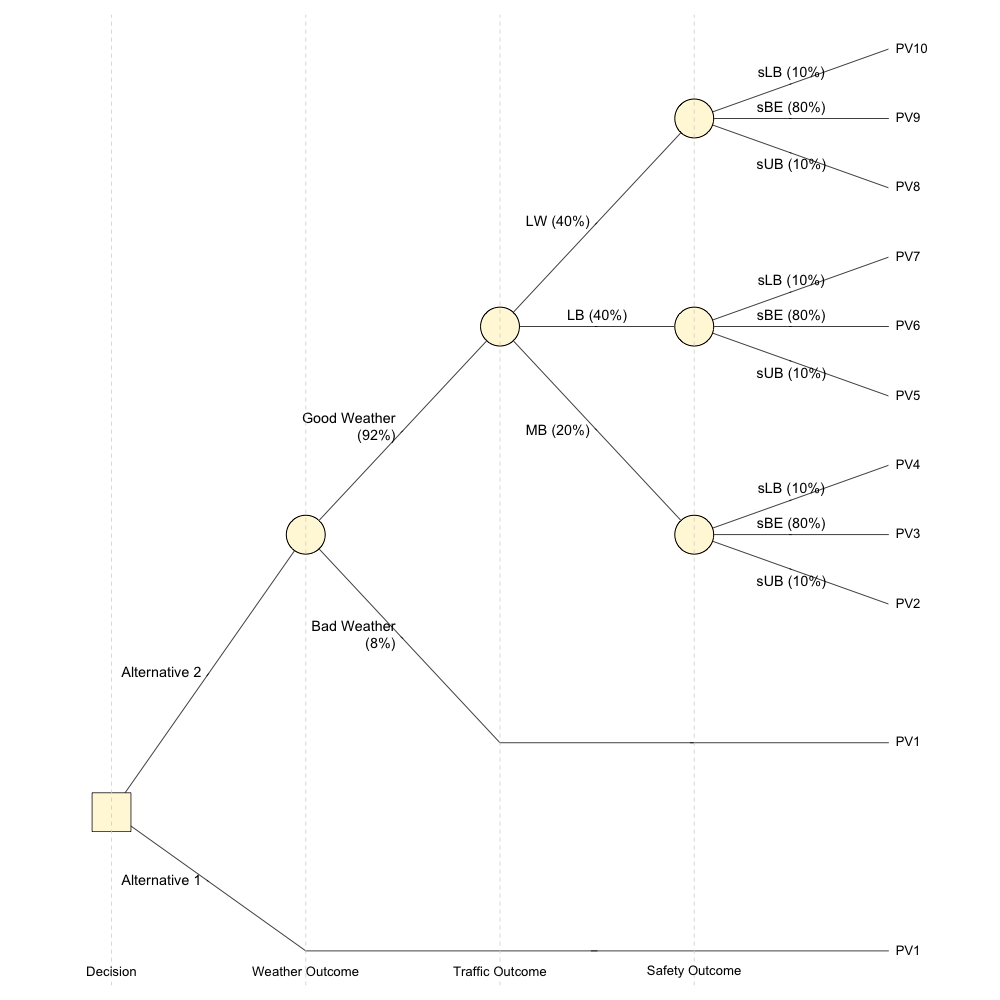
\includegraphics[width=0.7\textwidth]{../../R/decisiontree.png}
\caption{Representation of the problem as a decision tree. The square node represents the decision of choosing either alternative 1 or alternative 2. The circle nodes represent the uncertain events related to weather, traffic congestion or traffic safety. Alternative 3 could be interpreted as another branch in the decision node that would result in a new tree identical to the this one but with different probabilities for MB, LB, LW}
\label{decisiontree}
\end{figure}

\section{Analysis and Results} \label{results}

Table \ref{tab:results1} presents the resulting NPV for each alternative. For the reference case (Alternative 1) we can observe that the component that results in the largest cost is congestion. The total present value of costs for the reference case is approximately \$ 109 Billion. Implementation of AM (alternative 2) results in a decrease of the expected present value of costs of approximately \$ 2 Billion or 1.6\%. Most of the reduction is due to reduction in the congestion costs. On the other hand, the component cost that results in the biggest relative change is mortality costs, which are reduced by 3.9 \% (\$ 60 million).

\begin{table}[H]
\caption{NPV results for Alternative 1 and Alternative 2}
\vspace{0.5em}
\newcolumntype{x}[1]{>{\centering\arraybackslash\hspace{0pt}}p{#1}}
\newcolumntype{y}[1]{>{\centering\arraybackslash\hspace{0pt}}p{#1}}
\centering
\csvreader[
tabular=p{8em} x{6em} x{6em} x{6em} x{6em},
table head=\hline Name & Alternative 1 (Billion \$) & Alternative 2 (Billion \$) & Change (Billion \$) & Change (\%) \\\hline\hline,%
table foot=\hline\hline]%
{../../R/table_alternatives.csv}%
{name=\name, alt1=\firstalt, alt2=\secondalt, abschange=\abschange, percchange=\percchange}%
{\name & \firstalt & \secondalt & \abschange & \percchange}%
\label{tab:results1}
\end{table}%

To analyze whether choosing Alternative 3 (performing a pilot test) would be better than choosing Alternative 2 (which we already know is better than Alternative 1 without the test), we can compute the Net Expected Value of Imperfect Information (NEVII). This quantity would show the monetary value of this pilot test and already accounts for the actual cost of the test. Figure \ref{fig:evii} presents the NEVII for different values of the test size. We can observe that for small sizes of the test (< 50\% of the fleet), it aggregates no value to the decision maker. This means that the expected value of the decision with the test is the same as without the test (i.e., choosing alternative 2). As the test size increases, the value also increases, which means that the NPV with the test is larger than the NPV without the test. According to these results, the optimal test size is 100\% of the fleet.

\begin{figure}[h]
\centering
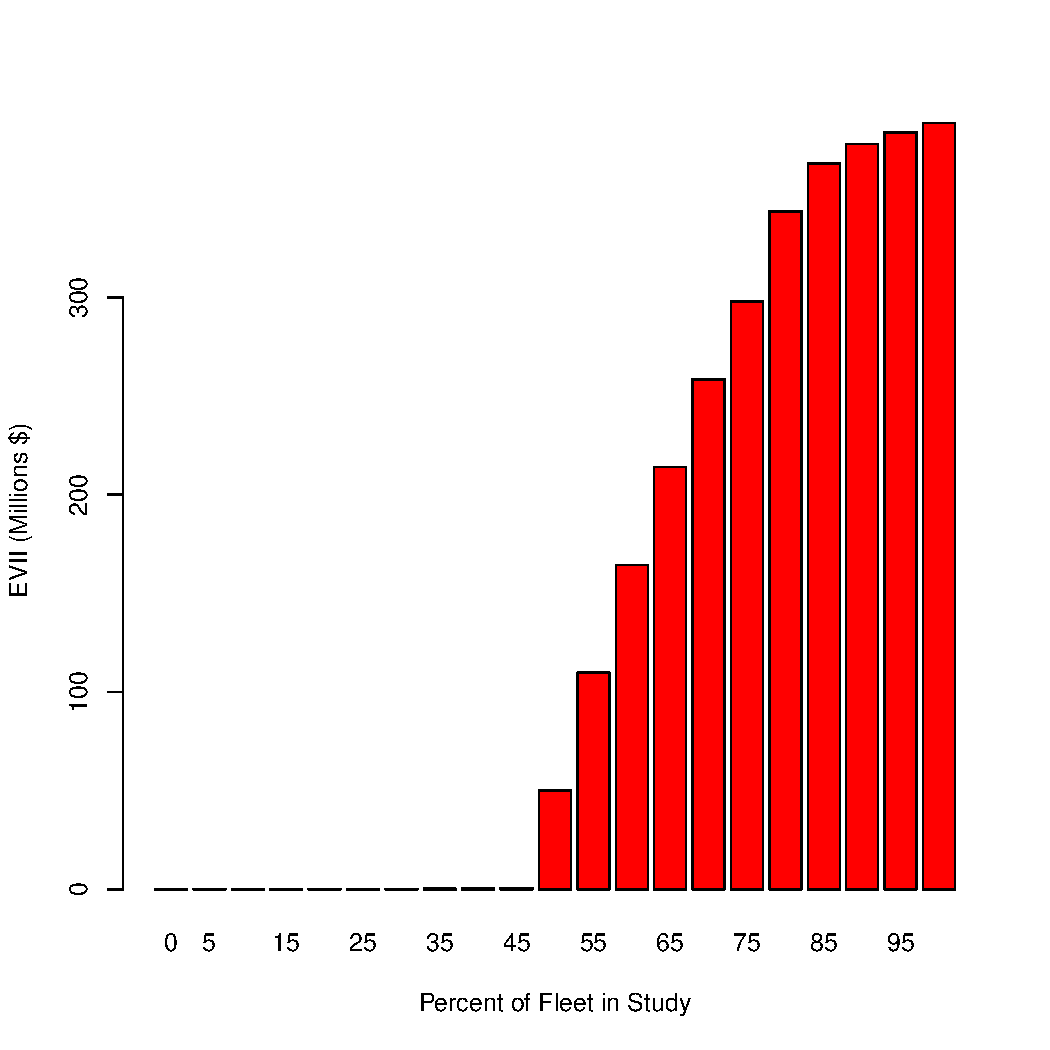
\includegraphics[width=0.45\textwidth]{../../R/alt3Barplot.pdf}
\caption{Net Expected Value of Imperfect Information}
\label{fig:evii}
\end{figure}



\section{Sensitivity Analysis} \label{sensitivity}

To perform the sensitivity analyses, we followed the methods used
above but varied key assumptions used in the original computation of
net expected values under uncertainty.  We varied the discount rate
from 2 to 12\% simply because these are the extreme values for this
figure.  While alternative 3 was the best choice under all discount
rates, the net expected NPV varied greatly under differing discount
rates. Similarly, alternative 3 had the least net expected cost under
all values used for lifetime and VSL.  Last, weather affected
alternatives 2 and 3 but not 1.  As the percent of weather
undrivable for AM increases, it becomes less cost effective; however,
without  weather patterns changing dramatically (precipitation more
than 50 of the time) alternatives 2 and 3 will continue to cost less
than alternative 1.

\begin{figure}[h]
\centering
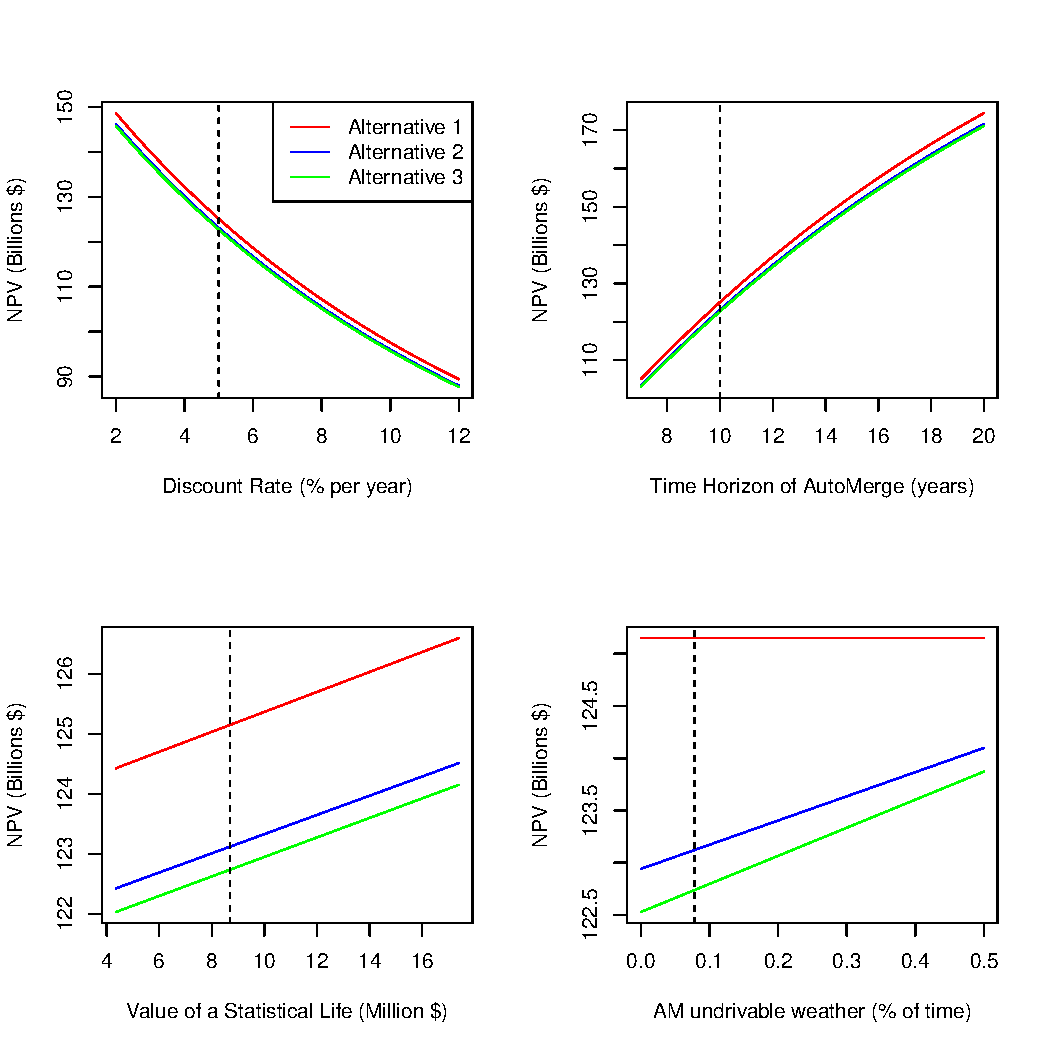
\includegraphics[width=0.8\textwidth]{../../R/sensitivity.pdf}
\caption{The figure above shows the impact of discount rate, lifetime
  of AM, value of a statistical life, and weather conditions on
  expected net NPV.  The vertical dashed line indicates our
  assumptions from the main analysis}
\label{fig:sensitivity}
\end{figure}

\section{Discussion} \label{discussion}

%\todo[inline]{Write discussion.}

\section{Conclusion \& Recommendations} \label{conclusion}

%\todo[inline]{Write Conclusion and Recommendations.}

\pagebreak
\pagebreak
\begin{multicols}{2}
\printbibliography[heading=none]
\end{multicols}

\end{document}
